\documentclass[tikz]{standalone}
\usepackage{amssymb,dsfont}
\usepackage{color}
\usetikzlibrary{arrows}
% Sets
\newcommand{\CC}{\mathbb{C}}        % Complex numbers
\newcommand{\NN}{\mathbb{N}}        % Natural numbers
\newcommand{\RR}{\mathbb{R}}        % Real numbers
\newcommand{\ZZ}{\mathbb{Z}}        % Relative integers
% Groups
\newcommand{\SO}{\mathrm{SO}}       % Special orthogonal group
\newcommand{\OO}{\mathrm{O}}        % Orthogonal group
\newcommand{\SU}{\mathrm{SU}}       % Special unitary group
\newcommand{\1}{\mathds{1}}		    % trivial group
\newcommand{\DD}{\mathbb{D}}        % Dihedral group
\newcommand{\octa}{\mathbb{O}}      % Cubic (octahedral) group
\newcommand{\ico}{\mathbb{I}}       % Icosahedral group
\newcommand{\tetra}{\mathbb{T}}     % tetrahedral group
\begin{document}
	
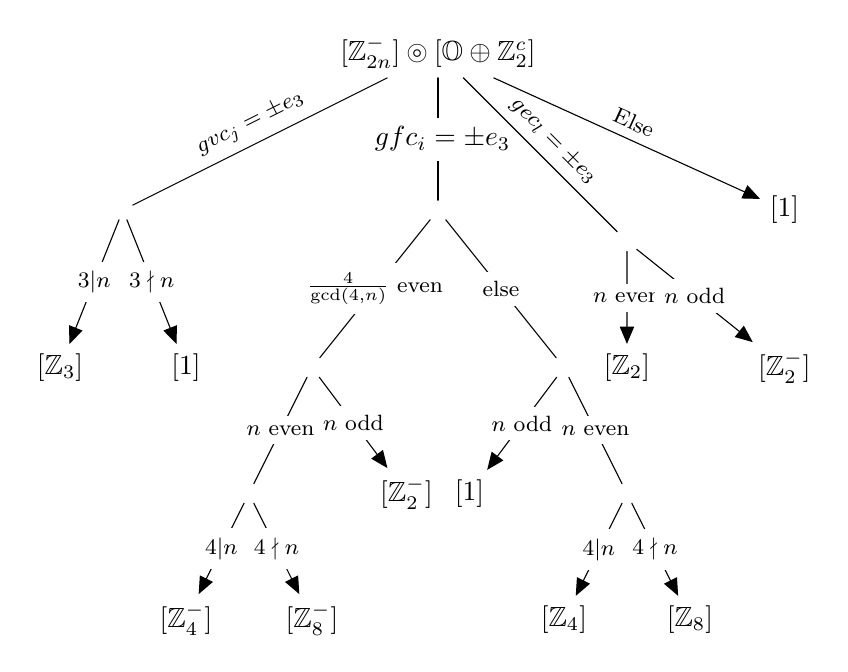
\begin{tikzpicture}[scale=0.8,line cap=round,line join=round,>=triangle 45,x=1.0cm,y=1.0cm]
  \node (root) at (0,0) {$[\ZZ_{2n}^-]\circledcirc [\octa\oplus \ZZ_2^c]$};

  \node (Bas1) at (-5,-2.5) {};
  \node (Bas2) at (0,-2.5)   {};
  \node (Bas3) at (3,-3)   {};
  \node (Bas4) at (5.5,-2.5) {$[\1]$};
  \draw (root) -- (Bas1) node [midway,above,sloped] {{\footnotesize  $gvc_j=\pm e_3$}};
  \draw (root) -- (Bas2) node [midway,fill=white] {{ $gfc_i=\pm e_3$ }};
  \draw (root) -- (Bas3) node [midway,above,sloped] {{\footnotesize  $gec_l=\pm e_3$}};
  \draw[->] (root) -- (Bas4) node [midway,above,sloped] {{\footnotesize  Else}};
   \node (Bas11) at (-5-1,-5) {$[\ZZ_3]$};
  \node (Bas12) at (-5+1,-5)  {$[\1]$};
  \draw[->] (Bas1) -- (Bas11) node [midway,fill=white] {{\footnotesize  $3|n$}};
  \draw[->] (Bas1) -- (Bas12) node [midway,fill=white] {{\footnotesize  $3\nmid n$}};
  \node (Bas21) at (0-2,-5) {};
  \node (Bas22) at (0+2,-5){} ;
  \draw (Bas2) -- (Bas21) node [midway,fill=white] {{\footnotesize  $\frac{4}{\gcd(4,n)}$ even}};
  \draw (Bas2) -- (Bas22) node [midway,fill=white] {{\footnotesize  else}};
  \node (Bas211) at (-1-2,-7) {};
  \node (Bas212) at (-1+0.5,-7) {$[\ZZ_2^-]$};
  \draw (Bas21) -- (Bas211) node [midway,fill=white] {{\footnotesize  $n$ even}};
  \draw [->](Bas21) -- (Bas212) node [midway,fill=white] {{\footnotesize  $n$ odd}};
  \node (Bas2111) at (-4,-9) {$[\ZZ_4^-]$};
  \node (Bas2112) at (-2,-9) {$[\ZZ_8^-]$};
  \draw [->] (Bas211) -- (Bas2111) node [midway,fill=white] {{\footnotesize  $4|n$}};
  \draw [->](Bas211) -- (Bas2112) node [midway,fill=white] {{\footnotesize  $4 \nmid n$}};
  \node (Bas221) at (0.5,-7) {$[\1]$};
  \node (Bas222) at (2+1,-7) {};
  \draw [->] (Bas22) -- (Bas221) node [midway,fill=white] {{\footnotesize  $n$ odd}};
  \draw  (Bas22) -- (Bas222) node [midway,fill=white] {{\footnotesize  $n$ even}};
  \node (Bas2221) at (3-1,-9) {$[\ZZ_4]$};
  \node (Bas2222) at (3+1,-9) {$[\ZZ_8]$};
  \draw [->] (Bas222) -- (Bas2221) node [midway,fill=white] {{\footnotesize  $4|n$}};
  \draw [->](Bas222) -- (Bas2222) node [midway,fill=white] {{\footnotesize  $4 \nmid n$}};
  \node (Bas31) at (3,-5) {$[\ZZ_2]$};
  \node (Bas32) at (3+2.5,-5)  {$[\ZZ_2^-]$};
  \draw[->] (Bas3) -- (Bas31) node [midway,fill=white] {{\footnotesize  $n$ even}};
  \draw[->] (Bas3) -- (Bas32) node [midway,fill=white] {{\footnotesize  $n$ odd}};
\end{tikzpicture}
% Further ’tikzpicture’ environments are possible which will create further pages.
\end{document} 